\question[20] An elevator is accelerating upward at a rate of $a=3.6$ m/s$^2$. A block of mass $m_1=75$ kg hangs by a low-mass rope from the ceiling, and another block of mass $m_2=22$ kg hangs by a low-mass rope from the upper block.

What are the tensions in the upper and lower ropes?
\begin{center}
	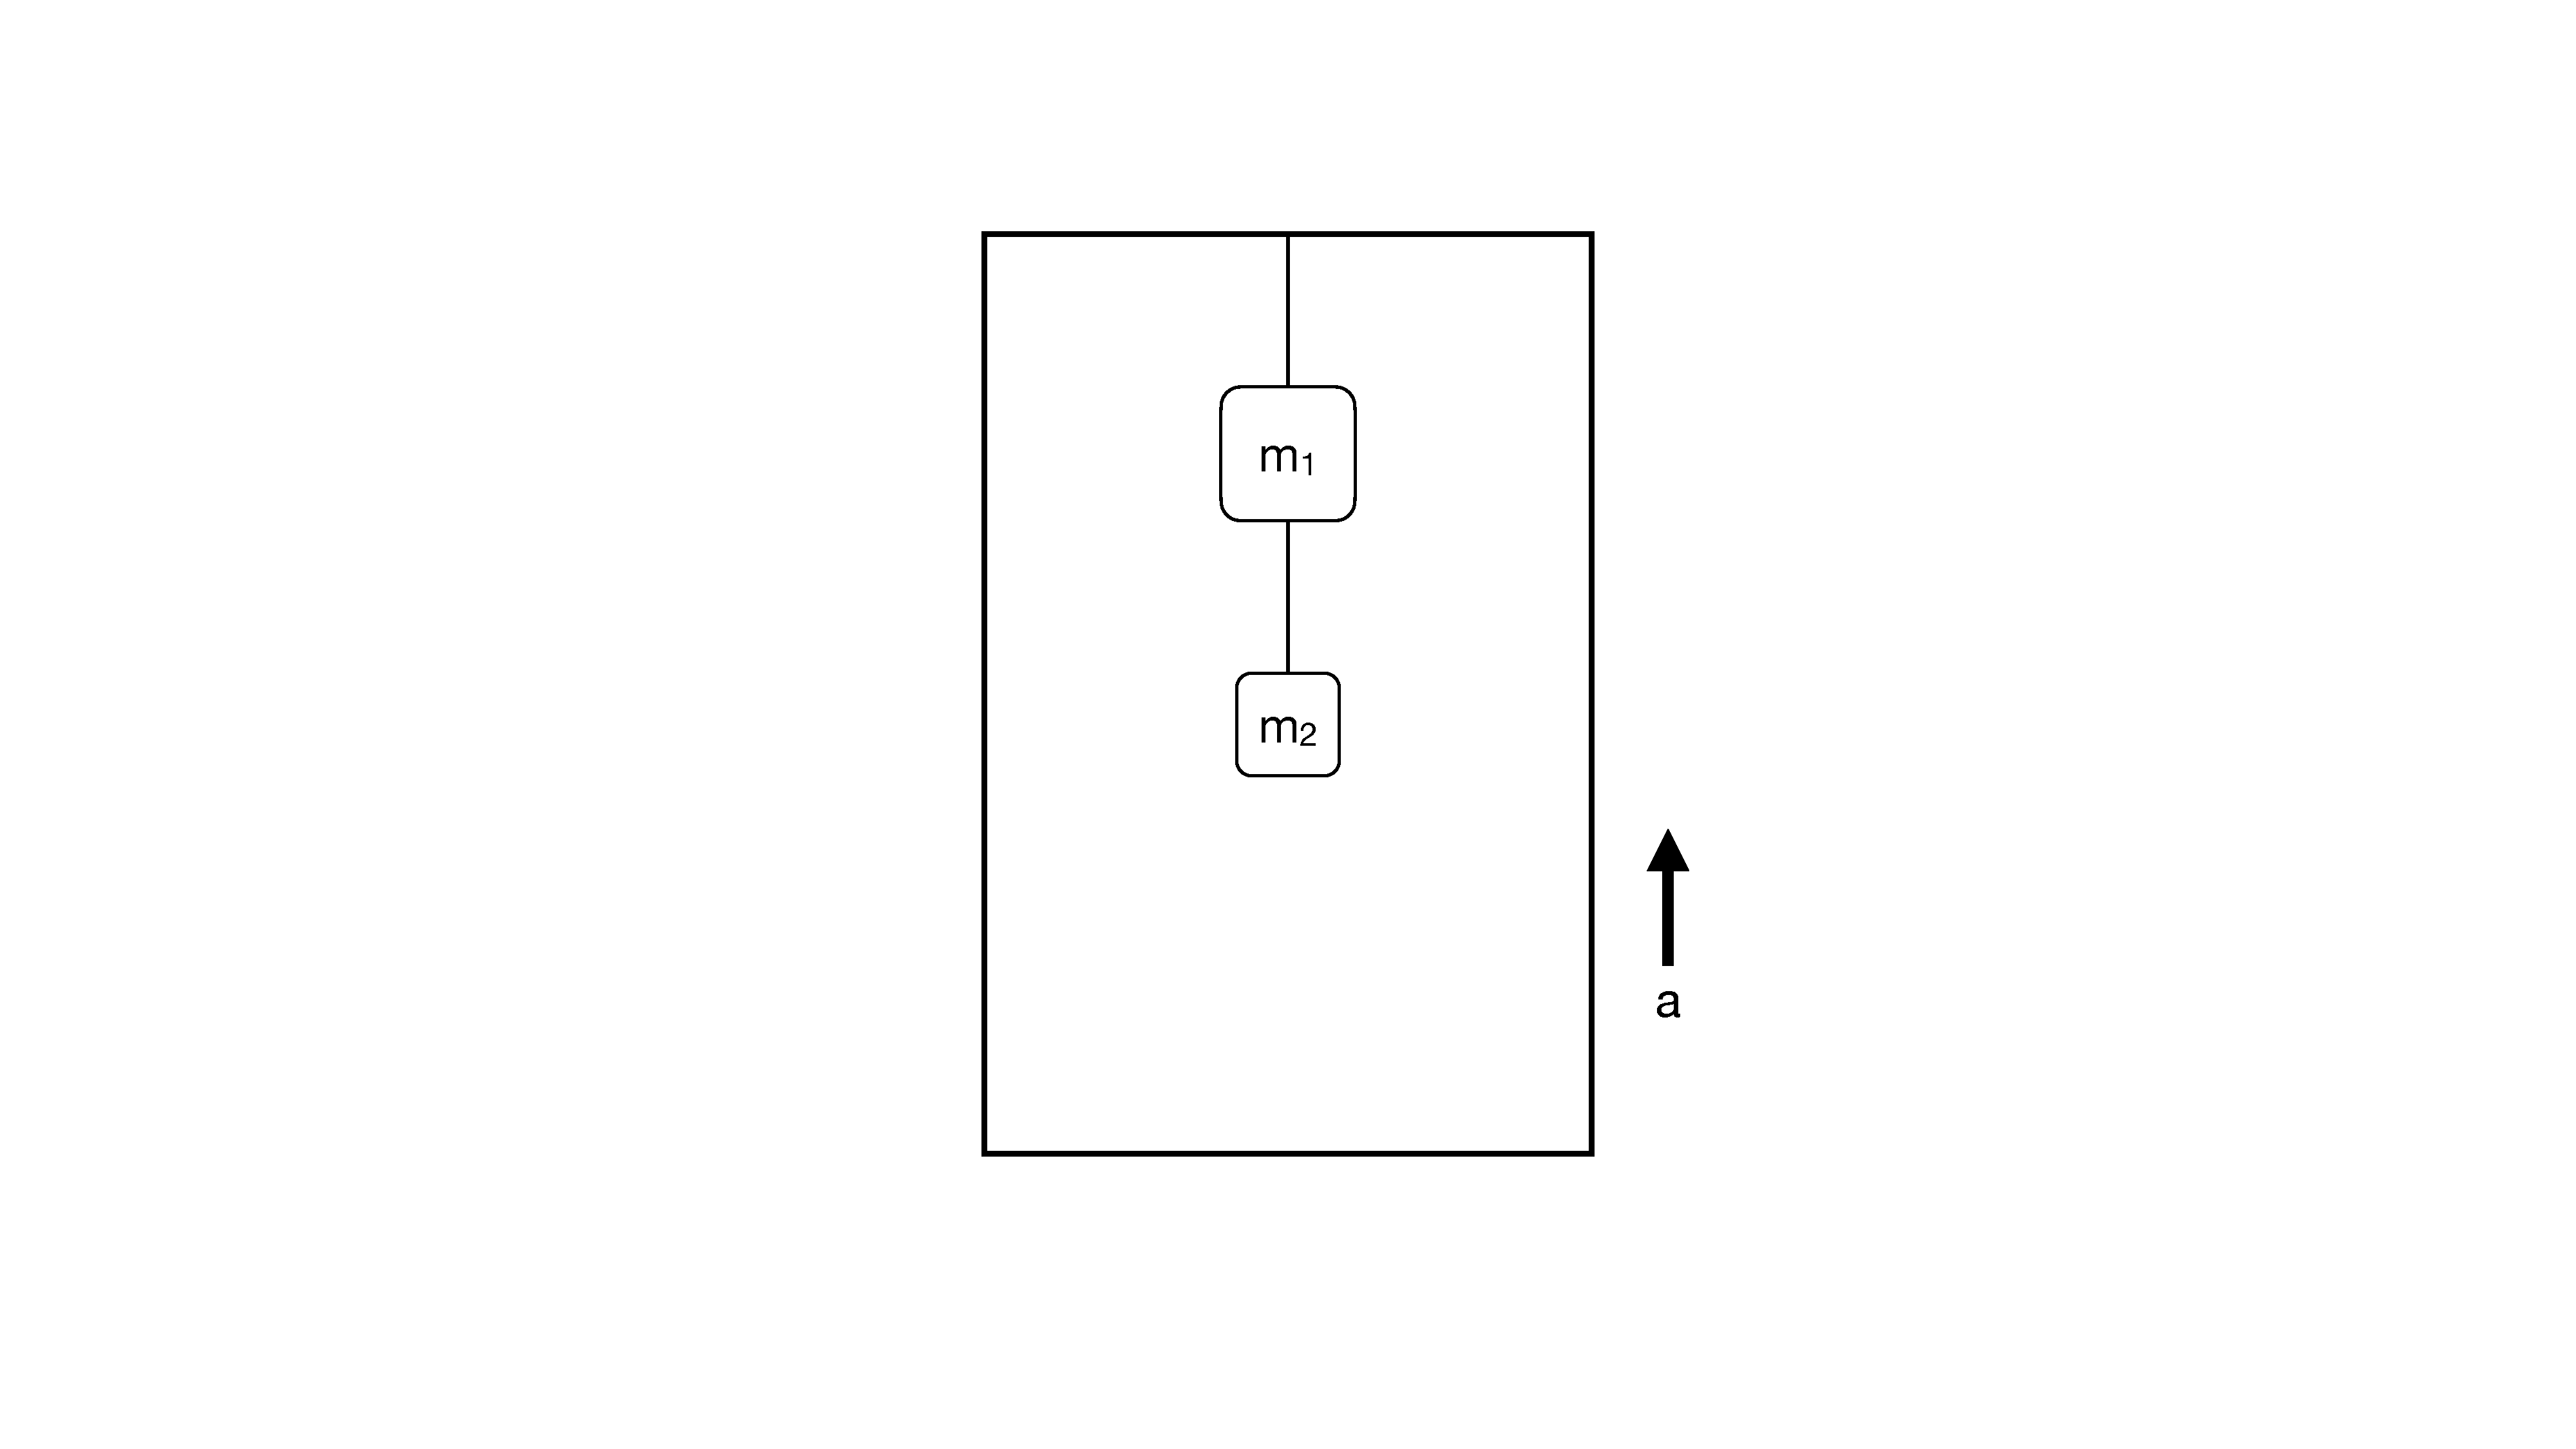
\includegraphics[width=5cm]{tension.pdf}
\end{center}
